\documentclass[12pt]{article}
\usepackage[margin=1in]{geometry}
\usepackage{amsmath,amsthm,amssymb,epigraph,etoolbox,mathtools,setspace,enumitem} 
\usepackage{tikz}
\usetikzlibrary{datavisualization}
\usepackage[makeroom]{cancel} 
\usepackage[linguistics]{forest}
\usetikzlibrary{patterns}
\newcommand{\N}{\mathbb{N}}
\newcommand{\Z}{\mathbb{Z}}
\newcommand{\R}{\mathbb{R}}
\newcommand{\Q}{\mathbb{Q}}

\newenvironment{theorem}[2][Theorem]{\begin{trivlist}
		\item[\hskip \labelsep {\bfseries #1}\hskip \labelsep {\bfseries #2.}]}{\end{trivlist}}
\newenvironment{lemma}[2][Lemma]{\begin{trivlist}
		\item[\hskip \labelsep {\bfseries #1}\hskip \labelsep {\bfseries #2.}]}{\end{trivlist}}
\newenvironment{exercise}[2][Exercise]{\begin{trivlist}
		\item[\hskip \labelsep {\bfseries #1}\hskip \labelsep {\bfseries #2.}]}{\end{trivlist}}
\newenvironment{problem}[2][Problem]{\begin{trivlist}
		\item[\hskip \labelsep {\bfseries #1}\hskip \labelsep {\bfseries #2.}]}{\end{trivlist}}
\newenvironment{question}[2][Question]{\begin{trivlist}
		\item[\hskip \labelsep {\bfseries #1}\hskip \labelsep {\bfseries #2.}]}{\end{trivlist}}
\newenvironment{corollary}[2][Corollary]{\begin{trivlist}
		\item[\hskip \labelsep {\bfseries #1}\hskip \labelsep {\bfseries #2.}]}{\end{trivlist}}
\newenvironment{solution}[2][Solution]{\begin{trivlist}
		\item[\hskip \labelsep {\bfseries #1}\hskip \labelsep {\bfseries #2.}]}{\end{trivlist}}

\setlength\epigraphwidth{8cm}
\setlength\epigraphrule{0pt}

\makeatletter
\patchcmd{\epigraph}{\@epitext{#1}}{\itshape\@epitext{#1}}{}{}
\makeatother


\begin{document}
	
	\title{Week 8}
	\author{Juan Patricio Carrizales Torres \\
		Section 6: Cartesian Products of Sets}
	\date{September 14, 2021}
	\maketitle
 
\begin{problem}{62}
	Describe the graph of the circle whose equation is $x^{2} + y^{2} = 4$ as a subset of $\R \times \R$.
	\begin{solution}{}
	The graph of the equation $x^{2}+y^{2}=4$ is the set $C=\{(x,y)\in \R \times \R: x^{2}+y^{2}=4\}$. The set $C \subset \R^{2}$.
	\end{solution}
\end{problem}

\begin{problem}{63}
	List the elements of the set $S=\{(x,y)\in \Z\times \Z: |x|+|y|=3\}$. Plot the corresponding points in the Euclidean $xy$-plane.
	\begin{solution}{}
		The set 
		\begin{align*}
		S &= \{(x,y)\in \Z\times \Z: |x|+|y|=3\}\\
		& = \{(1,2),(-1,2),(1,-2),(-1,-2),(3,0),(-3,0),(2,1),(-2,1),(2,-1),(-2,-1),(0,3),(0,-3)\}
		\end{align*}
	The next figure shows the plot of these points in the Euclidean $xy$-plane.\\
	\begin{center}
	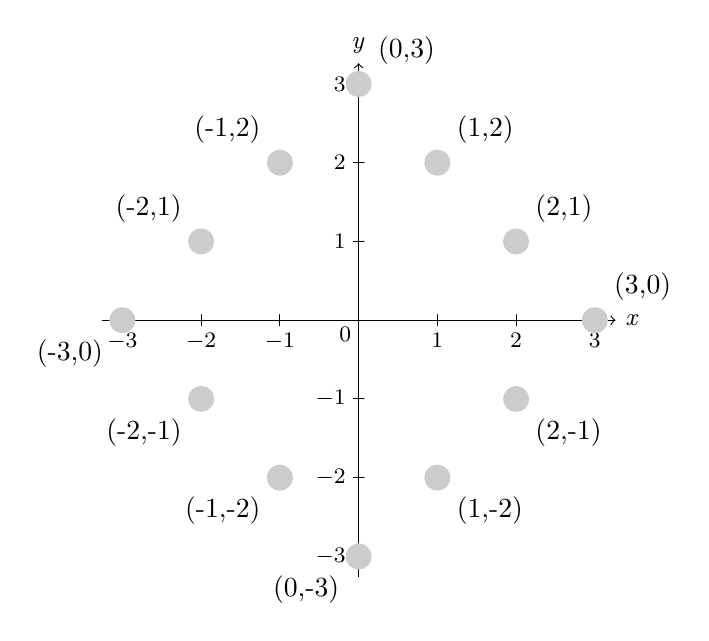
\begin{tikzpicture}
		[mycirc/.style={circle,fill=black!20, minimum size=0.001cm}
		]
	\datavisualization [school book axes,
	visualize as smooth line,
	y axis={label,min value = -3, max value = 3},
	x axis={label, min value = -3, max value = 3} ];
	\node[mycirc, label=above right:{(1,2)}] at (1,2) {};
	\node[mycirc, label=above left:{(-1,2)}] at (-1,2) {};
	\node[mycirc, label=below right:{(1,-2)}] at (1,-2) {};
	\node[mycirc, label=below left:{(-1,-2)}] at (-1,-2) {};
	\node[mycirc, label=above right:{(3,0)}] at (3,0) {};
	\node[mycirc, label=below left:{(-3,0)}] at (-3,0) {};
	\node[mycirc, label=above right:{(2,1)}] at (2,1) {};
	\node[mycirc, label=above left:{(-2,1)}] at (-2,1) {};
	\node[mycirc, label=below right:{(2,-1)}] at (2,-1) {};
	\node[mycirc, label=below left:{(-2,-1)}] at (-2,-1) {};
	\node[mycirc, label=above right:{(0,3)}] at (0,3) {};
	\node[mycirc, label=below left:{(0,-3)}] at (0,-3) {};
	\end{tikzpicture}
	\end{center}
	\end{solution}
\end{problem}

\begin{problem}{64}
	For $A = \{1,2\}$ and $B=\{1\}$, determine $\mathcal{P}(A\times B)$.
	\begin{solution}{}
		The set $A\times B = \{(1,1),(2,1)\}$. Since $|A\times B| = 2$, it follows that $|\mathcal{P}(A\times B)|= 2^{2}=4$. The set $\mathcal{P}(A\times B) = \{\emptyset,\{(1,1)\},\{(2,1)\},A\times B\}$.
	\end{solution}
\end{problem}

\begin{problem}{65}
	For $A=\{x\in \R:|x-1|\leq 2\}$ and $B=\{y\in \R: |y-4|\leq 2\}$, give a geometric description of the points in the $xy$-plane belonging to $A\times B$.
	\begin{solution}{}
		The sets $A=[-1,3]$ and $B=[2,6]$. Since the cartesian product $A\times B= \{(a,b):a\in [-1,3] \text{ and } b\in [2,6]\}$, it follows that the points in $A\times B$ are found on and inside the square bounded by $x=-1$, $x=3$, $y=2$ and $y=6$ (Note that each side is of length 4 units).
	\end{solution}
\end{problem} 
   
\begin{problem}{66}
	For $A=\{a \in \R:|a|\leq 1\}$ and $B=\{b\in \R: |b|=1\}$, give a geometric description of the points in the $xy$-plane belonging to $(A\times B)\cup(B\times A)$
	\begin{solution}{}
		The sets $A=[-1,1]$ and $B=\{-1,1\}$. Each point in $A\times B = [-1,1]\times \{-1,1\}$ lies on one of the two horizontal parallel lines $y=-1$ and $y=1$ with $x\in [-1,1]$. Also, each point in $B\times A = \{-1,1\}\times [-1,1]$  lies on one of the two vertical parallel lines $x=-1$ and $x=1$ with $y \in [-1,1]$. Thus, all the points belonging to $(A\times B)\cup(B\times A)$ lie just on (not inside) the square bounded by $x=-1$, $x=1$, $y=-1$ and $y=1$.
	\end{solution}
\end{problem}
\end{document}